\documentclass[11pt,a4paper]{article}

% ----- Page layout -----
\usepackage[a4paper,margin=2.5cm]{geometry}
\usepackage{parskip}
\usepackage{microtype}

% ----- Math -----
\usepackage{amsmath,amssymb,amsfonts}
\usepackage{mathtools}
\usepackage{bm}
\usepackage{siunitx}
  \sisetup{per-mode=symbol, separate-uncertainty=true}

% ----- Graphics & figures -----
\usepackage{graphicx}
\usepackage{float}
\usepackage{caption}
\captionsetup{font=small,labelfont=bf,skip=4pt}
\usepackage{subcaption}

% ----- TikZ / CircuiTikZ -----
\usepackage{tikz}
\usepackage{circuitikz}
\usetikzlibrary{calc,arrows.meta,positioning,decorations.pathmorphing}

% ----- Tables -----
\usepackage{booktabs}
\usepackage{array}
\usepackage{tabularx}

% ----- Headers, hyperlinks, colors -----
\usepackage{xcolor}
\usepackage{hyperref}
\hypersetup{
  colorlinks=true,
  linkcolor=blue!60!black,
  urlcolor=blue!60!black,
  citecolor=blue!60!black
}
\usepackage{fancyhdr}
\pagestyle{fancy}
\fancyhf{}
\fancyhead[L]{\small ET4260 -- Microsystems Design and Modelling}
\fancyhead[R]{\small Final assignment, Part 1/3}
\fancyfoot[C]{\thepage}
\renewcommand{\headrulewidth}{0.4pt}

% ----- Custom commands -----
\newcommand{\Vd}{V_{d}}
\newcommand{\VDC}{V_{\mathrm{DC}}}
\newcommand{\VAC}{V_{\mathrm{AC}}}
\newcommand{\xm}{x_{m}}
\newcommand{\Fe}{F_{e}}
\newcommand{\Fd}{F_{d}}
\newcommand{\geff}{g_{\mathrm{eff}}}
\newcommand{\neff}{n_{\mathrm{eff}}}

% ----- Title block -----
\title{\vspace{-1.5cm}
  \textbf{Final assignment -- Part 1/3} \\[2pt]
  \large Microsystems Design and Modelling (ET4260)}
\author{Daniel Tyukov \\ Student number: 5714699}
\date{First submission: 13\textsuperscript{th} May 2026}

\begin{document}

% ===================== Title page =====================
\begin{titlepage}
\centering
\vspace*{1cm}
{\large\textbf{DELFT UNIVERSITY OF TECHNOLOGY}}\\[2pt]
{\small Faculty of Electrical Engineering, Mathematics and Computer Science}\\[2cm]

\includegraphics[width=0.25\textwidth]{figures/tudelft_logo.jpeg}\\[2cm]
{\Large\textbf{Final assignment}}\\[6pt]
{\Large\textbf{Microsystems Design and Modelling (ET4260)}}\\[6pt]
{\Large\textbf{Part 1/3}}\\[1.5cm]

\begin{minipage}{0.85\textwidth}
\centering\small
\textbf{Instructions.} Document your calculations properly with derivations and screenshots when needed.
Latex-generated PDF files are accepted.\\[6pt]
Deadline for first submission of Part 1: 13\textsuperscript{th} May 2026.\\
Deadline for final report submission: 24\textsuperscript{th} June 2026.\\
Corrections made after the first submission are marked in \textcolor{blue}{blue}.
\end{minipage}
\vfill
\rule{0.7\textwidth}{0.4pt}\\[4pt]
{\large Daniel Tyukov}\\[2pt]
{\large Student number: 5714699}\\[4pt]
\rule{0.7\textwidth}{0.4pt}
\vspace{1cm}
\end{titlepage}

% ===================== Device introduction =====================
\section*{Optical phase shifter for quantum applications}
\addcontentsline{toc}{section}{Device overview}

The MEMS photonic phase shifter studied in this report (Fig.~\ref{fig:schematic}) modulates the
optical phase by changing the gap $g$ between a suspended silicon mass and an
adjacent waveguide. The mass is suspended by four fixed--guided beams and
displaced by a comb-drive actuator biased with $\Vd$. With the gap varying as
$g=g_{0}+\xm$, the additional phase shift is
\begin{equation}
  \Delta\phi(g) = \frac{2\pi L}{\lambda}\,\bigl(\neff(g_{0}) - \neff(g)\bigr),
  \qquad
  \neff(g) = (\eta_{\mathrm{eff},0}-\eta_{\mathrm{eff},\infty})\,e^{-bg} + \eta_{\mathrm{eff},\infty}.
  \label{eq:phase}
\end{equation}

\begin{figure}[H]
\centering
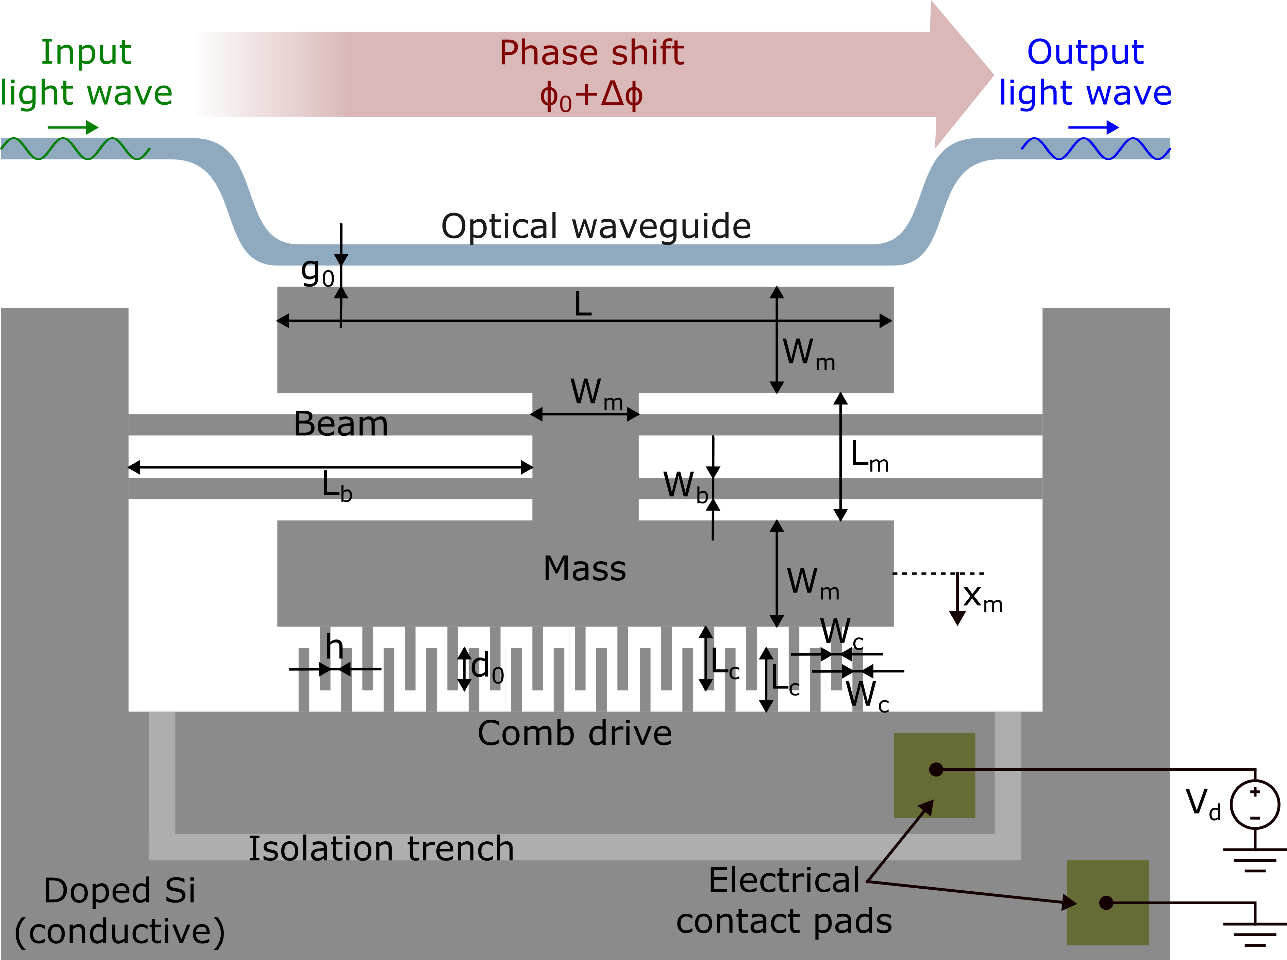
\includegraphics[width=0.78\textwidth]{figures/schematic.png}
\caption{Schematic of the MEMS optical phase shifter (top view, not to scale).
The waveguide sits a gap $g_{0}$ above the modulation section.
The central mass is suspended by four fixed--guided beams of length $L_{b}$
and width $W_{b}$, anchored on either side. The comb drive at the bottom
generates the actuating force $\Fe$.}
\label{fig:schematic}
\end{figure}

\begin{table}[H]
\centering
\small
\caption{Design parameters used throughout this report.}
\label{tab:params}
\begin{tabularx}{0.85\textwidth}{l l X}
\toprule
\textbf{Symbol} & \textbf{Value} & \textbf{Description}\\
\midrule
$L$        & \SI{100}{\micro\meter}  & length of modulation section\\
$g_{0}$    & \SI{200}{\nano\meter}   & modulation gap at rest\\
$L_{b}$    & \SI{75}{\micro\meter}   & beam length\\
$W_{b}$    & \SI{5}{\micro\meter}    & beam width\\
$L_{m}$    & \SI{40}{\micro\meter}   & mass central section length\\
$W_{m}$    & \SI{30}{\micro\meter}   & mass section width\\
$h$        & \SI{1}{\micro\meter}    & comb-drive gap\\
$d_{0}$    & \SI{19}{\micro\meter}   & comb overlap at rest\\
$L_{c}$    & \SI{20}{\micro\meter}   & comb-finger length\\
$W_{c}$    & \SI{1}{\micro\meter}    & comb-finger width\\
$t$        & \SI{200}{\nano\meter}   & thickness of suspended layer\\
$N$        & 40                      & number of comb-drive gaps\\
$E_{Si}$   & \SI{170}{\giga\pascal}  & Young's modulus of silicon\\
$\rho_{Si}$& \SI{2330}{\kilo\gram\per\cubic\meter} & density of silicon\\
$\lambda$  & \SI{1550}{\nano\meter}  & optical wavelength\\
$b$        & \SI{0.3}{\per\micro\meter} & refractive-index decay constant\\
$\eta_{\mathrm{eff},0}$    & 2.6 & $\neff$ at $g=0$\\
$\eta_{\mathrm{eff},\infty}$ & 2.4 & $\neff$ as $g\to\infty$\\
$c_{\mathrm{air}}$ & \SI{16.15}{\newton\second\per\meter\cubed} & air damping coefficient\\
$Q_{\mathrm{clamping}}$ & 500 & clamping quality factor\\
\bottomrule
\end{tabularx}
\end{table}

\section{Mechanical model and dynamics}

\subsection*{Q1: Lumped-element equation of motion}

In vacuum and without damping, the suspended mass behaves as a single
spring-mass with input force $\Fe$ and output displacement $\xm$:
\begin{equation}
  m\,\ddot{\xm} + k\,\xm \;=\; \Fe.
  \label{eq:eom-undamped}
\end{equation}
Once air damping and clamping losses are included (Q4) the equation extends to
\begin{equation}
  m\,\ddot{\xm} + b\,\dot{\xm} + k\,\xm \;=\; \Fe,
  \label{eq:eom-damped}
\end{equation}
which is the classical mass-spring-damper system, equivalent to a series RLC
circuit (Fig.~\ref{fig:rlc}).

\begin{figure}[H]
\centering
\begin{circuitikz}[scale=0.95,transform shape]
  \draw (0,0)
    to[V,l=$\Fe$,invert] (0,3)
    to[L,l=$L\equiv m$] (3,3)
    to[R,l=$R\equiv b$] (6,3)
    to[C,l=$C\equiv 1/k$] (9,3)
    to[short] (9,0)
    to[short] (0,0);
\end{circuitikz}
\caption{Series-RLC equivalent circuit of the lumped mass-spring-damper
system. Effort $\leftrightarrow$ voltage, flow $\leftrightarrow$ current.}
\label{fig:rlc}
\end{figure}

\subsection*{Q2: Fundamental resonance frequency}

\paragraph{Stiffness.}
Each of the four beams is clamped at its anchor and connected to the rigid
mass at the other end. By the symmetry of the upper/lower beam pair, the
mass-side end translates without rotation, a \emph{fixed-guided} boundary
condition. Each beam therefore contributes
\begin{equation}
  k_{b} \;=\; \frac{12\,E_{Si}\,I}{L_{b}^{3}},
  \qquad
  I \;=\; \frac{t\,W_{b}^{3}}{12},
\end{equation}
where the in-plane width $W_{b}$ is the dimension along the bending
direction. With four beams in parallel,
\begin{equation}
  k \;=\; 4 k_{b} \;=\; \frac{4\,E_{Si}\,t\,W_{b}^{3}}{L_{b}^{3}}
        \;=\; \SI{40.30}{\newton\per\meter}.
\end{equation}

\paragraph{Effective mass.}
\textcolor{blue}{Neglecting the beam mass, the moving body is the suspended
silicon drawn in Fig.~\ref{fig:schematic}: the modulation bar, the central
column, the comb-spine plate that carries the fingers (the lower ``mass''
block) and the moving comb fingers. The geometry has \emph{two}
$L\times W_{m}$ plates, the modulation bar \emph{and} the comb spine, and
$20$ moving fingers, since $N=40$ counts the comb \emph{gaps}, not the
fingers:}
\begin{equation}
  m \;=\; \rho_{Si}\,t\bigl(\,\textcolor{blue}{2}\,L\,W_{m} + L_{m}\,W_{m}
        + \textcolor{blue}{20}\,L_{c}\,W_{c}\bigr)
        \;=\; \textcolor{blue}{\SI{3.54e-12}{\kilo\gram}}.
\end{equation}
\textcolor{blue}{The first submission counted only one plate and $N=40$
fingers, giving \SI{2.33e-12}{\kilo\gram}. Adding the missing comb spine and
using the correct finger count raises the mass by $1.5\times$ and brings this
analytical estimate close to the finite-element value of Part~2.}

\paragraph{Resonance.}
\begin{equation}
  \omega_{0}=\sqrt{\frac{k}{m}}=\textcolor{blue}{\SI{3.37e6}{\radian\per\second}},
  \qquad
  f_{0}=\frac{\omega_{0}}{2\pi}\approx \textcolor{blue}{\SI{537}{\kilo\hertz}}.
\end{equation}

\subsection*{Q3: Static deflection due to gravity}

With gravity acting along the direction of motion, static balance gives
\begin{equation}
  x_{g}=\frac{m\,g}{k}
       =\frac{\textcolor{blue}{\SI{3.54e-12}{\kilo\gram}}\cdot\SI{9.81}{\meter\per\second\squared}}
              {\SI{40.30}{\newton\per\meter}}
       \approx \textcolor{blue}{\SI{0.86}{\pico\meter}}.
\end{equation}
This is more than five orders of magnitude smaller than $g_{0}$. Gravity is
irrelevant at this scale; the comb-drive force dominates by a wide margin.

\section{Damping, settling time and shock tolerance}

\subsection*{Q4 -- Settling time with combined damping}

Independent loss channels add in parallel: damping coefficients sum, quality
factors combine as reciprocals.

\paragraph{Air damping.} The top-side area of the moving structure
\textcolor{blue}{(the same two plates, column and $20$ fingers used for the
mass)} is
\begin{equation}
  A_{m}=\textcolor{blue}{2}L W_{m} + L_{m} W_{m} + \textcolor{blue}{20}\, L_{c} W_{c}
      = \textcolor{blue}{\SI{7.60e-9}{\meter\squared}},
\end{equation}
giving an air damping coefficient
\begin{equation}
  b_{\mathrm{air}}=c_{\mathrm{air}}\,A_{m}=\textcolor{blue}{\SI{1.23e-7}{\newton\second\per\meter}},
  \qquad
  Q_{\mathrm{air}}=\frac{\sqrt{km}}{b_{\mathrm{air}}}=\textcolor{blue}{97}.
\end{equation}

\paragraph{Clamping loss.} From the given $Q_{\mathrm{clamping}}=500$,
\begin{equation}
  b_{\mathrm{clamp}}=\frac{\sqrt{km}}{Q_{\mathrm{clamping}}}
                   =\textcolor{blue}{\SI{2.39e-8}{\newton\second\per\meter}}.
\end{equation}

\paragraph{Combined damping.}
\begin{equation}
  b=b_{\mathrm{air}}+b_{\mathrm{clamp}}=\textcolor{blue}{\SI{1.47e-7}{\newton\second\per\meter}},
  \qquad
  \frac{1}{Q}=\frac{1}{Q_{\mathrm{air}}}+\frac{1}{Q_{\mathrm{clamping}}}
  \;\Rightarrow\; Q\approx \textcolor{blue}{81.5}.
\end{equation}
Air damping dominates (\textcolor{blue}{$Q_{\mathrm{air}}\!=\!97 \ll Q_{\mathrm{clamping}}\!=\!500$}),
so $Q$ is essentially set by the surrounding gas.
\textcolor{blue}{The corrected $Q\approx81.5$ is, reassuringly, close to the
$Q=83$ that Part~2 imposes on the FEM model.}

\paragraph{Settling time.} With \textcolor{blue}{$\zeta = b/(2\sqrt{km})=1/(2Q)\approx 6.1\times10^{-3}$}
the system is strongly underdamped. Its envelope decays as $e^{-\zeta\omega_{0}t}$,
giving a $\pm 5\%$ settling time of
\begin{equation}
  t_{s} \;\approx\; \frac{-\ln(0.05)}{\zeta\,\omega_{0}}
              \;=\; \frac{3.00}{\zeta\,\omega_{0}}
              \;\approx\; \textcolor{blue}{\SI{145}{\micro\second}}.
\end{equation}
Figure~\ref{fig:step} shows the simulated response for a 1\,nN step input.

\begin{figure}[H]
\centering
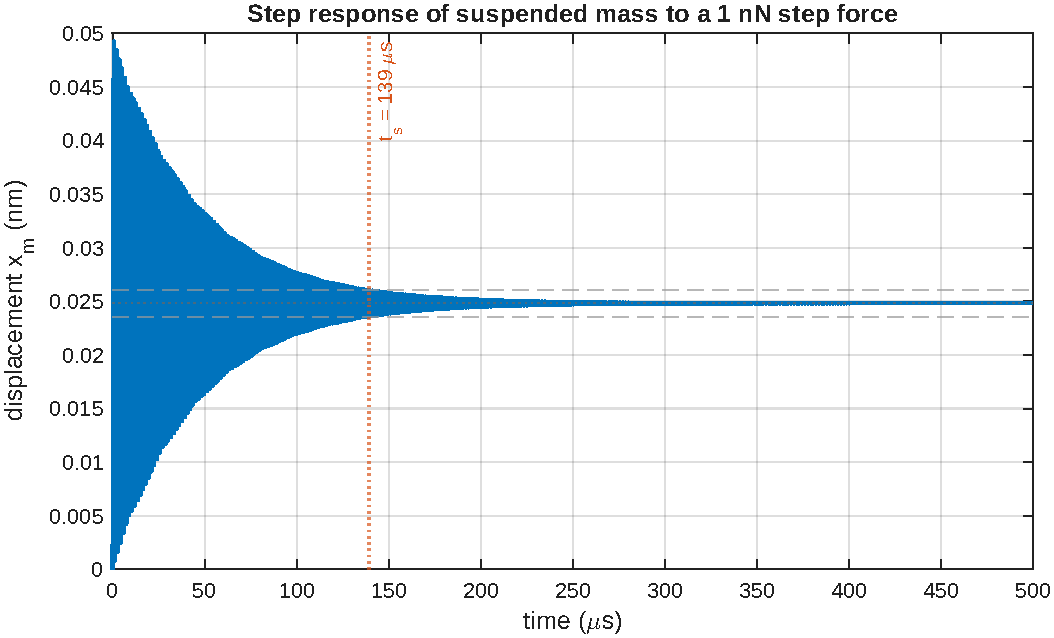
\includegraphics[width=0.78\textwidth]{figures/q4_step_response.pdf}
\caption{Step response to a 1\,nN input force. The dashed lines mark the
$\pm 5\%$ band around the steady-state value $F_{0}/k$. Settling occurs after
roughly $t_{s}\approx \textcolor{blue}{\SI{145}{\micro\second}}$.}
\label{fig:step}
\end{figure}

\subsection*{Q5 -- Maximum tolerable harmonic acceleration}

A harmonic base acceleration $a(t)=A\cos(\omega t)$ acts on the suspended mass
as an inertial force $-m a$. With $\Vd=0$ (no electrostatic force), the
equation of motion in the frequency domain is
\begin{equation}
  (k - m\omega^{2} + j\omega b)\,X(j\omega) = -m\,A(j\omega),
\end{equation}
so the magnitude of the displacement is
\begin{equation}
  |X(j\omega)| \;=\; \frac{m\,|A(j\omega)|}
                          {\sqrt{(k-m\omega^{2})^{2}+(\omega b)^{2}}}.
\end{equation}
The mass touches the waveguide when $|X|=g_{0}$. The maximum tolerable
acceleration as a function of frequency is therefore
\begin{equation}
  \boxed{\;
    A_{\max}(\omega) \;=\; \frac{g_{0}}{m}
      \sqrt{(k-m\omega^{2})^{2}+(\omega b)^{2}}.
  \;}
  \label{eq:Amax}
\end{equation}

\paragraph{DC limit ($\omega\to 0$).}
\begin{equation}
  A_{\max,\mathrm{DC}} \;=\; \frac{g_{0} k}{m} \;=\; g_{0}\,\omega_{0}^{2}
   \;\approx\; \textcolor{blue}{\SI{2.28e6}{\meter\per\second\squared}}
   \;\approx\; \textcolor{blue}{\SI{2.3e5}{\textit{g}}}.
\end{equation}

\paragraph{Worst-case AC frequency ($\omega = \omega_{0}$).} At resonance the
square root reduces to $\omega_{0} b$, so
\begin{equation}
  A_{\max,\mathrm{res}} \;=\; \frac{g_{0}\,\omega_{0}\,b}{m}
                          \;=\; \frac{g_{0}\,\omega_{0}^{2}}{Q}
                          \;\approx\; \textcolor{blue}{\SI{2.79e4}{\meter\per\second\squared}}
                          \;\approx\; \textcolor{blue}{\SI{2.8e3}{\textit{g}}}.
\end{equation}
Resonance reduces shock tolerance by a factor $Q$. The DC value
($\sim\!10^{5}\,g$) is enormous, but at $f_{0}$ the device is roughly
\textcolor{blue}{$80\times$} more vulnerable. Fig.~\ref{fig:amax} plots $A_{\max}(f)$.

\begin{figure}[H]
\centering
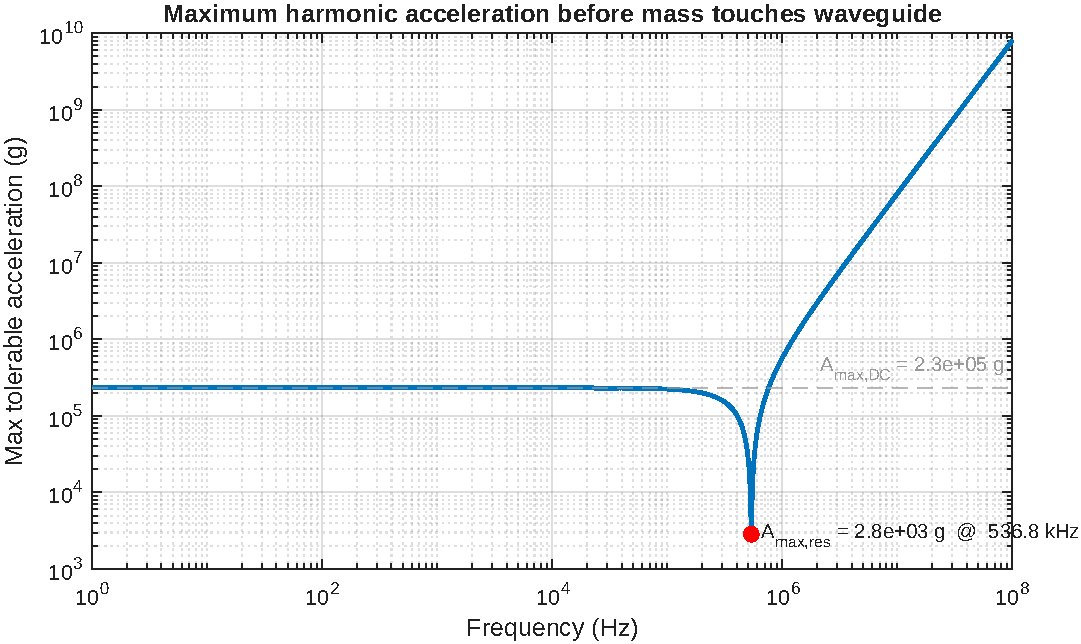
\includegraphics[width=0.78\textwidth]{figures/q5_amax.pdf}
\caption{Maximum tolerable acceleration before the suspended mass contacts
the waveguide, computed from Eq.~\ref{eq:Amax}. The minimum lies at
$f_{0}\approx \textcolor{blue}{\SI{537}{\kilo\hertz}}$, where the device is most sensitive to
mechanical excitation.}
\label{fig:amax}
\end{figure}

\section{Electrostatic transduction and sensitivity}

\subsection*{Q6: Static phase shift versus DC voltage}

Considering only the perpendicular field component, the comb-drive
capacitance varies linearly with the engagement length $d_{0}+\xm$:
\begin{equation}
  C(\xm) = N\,\varepsilon_{0}\,\frac{t\,(d_{0}+\xm)}{h},
  \qquad
  \frac{dC}{d\xm} = \frac{N\,\varepsilon_{0}\,t}{h}
                  = \SI{7.08e-11}{\farad\per\meter}.
\end{equation}
The electrostatic force on the mass therefore depends only on voltage:
\begin{equation}
  \Fe = \tfrac{1}{2}\,\Vd^{2}\,\frac{dC}{d\xm}
      = \tfrac{1}{2}\,\Vd^{2}\,\frac{N\,\varepsilon_{0}\,t}{h}.
  \label{eq:Fcomb}
\end{equation}
Static balance with the spring force ($\Fe=k\xm$) yields the displacement
\begin{equation}
  \xm(\Vd) \;=\; \frac{\Vd^{2}\,N\,\varepsilon_{0}\,t}{2 k h},
  \qquad
  g(\Vd) \;=\; g_{0} + \xm(\Vd).
  \label{eq:gV}
\end{equation}
Substituting into Eq.~\ref{eq:phase} gives the phase shift plotted in
Fig.~\ref{fig:q6}. It is symmetric in $\Vd$ and quadratic. At
$\Vd=\pm 50\,\mathrm{V}$ the gap only changes by $\xm\approx \SI{2.2}{\nano\meter}$
(1\% of $g_{0}$), so $|\Delta\phi|$ stays around $\SI{50}{\milli\radian}$. Reaching
$\pi$ radians of phase shift would need a much higher bias.

\begin{figure}[H]
\centering
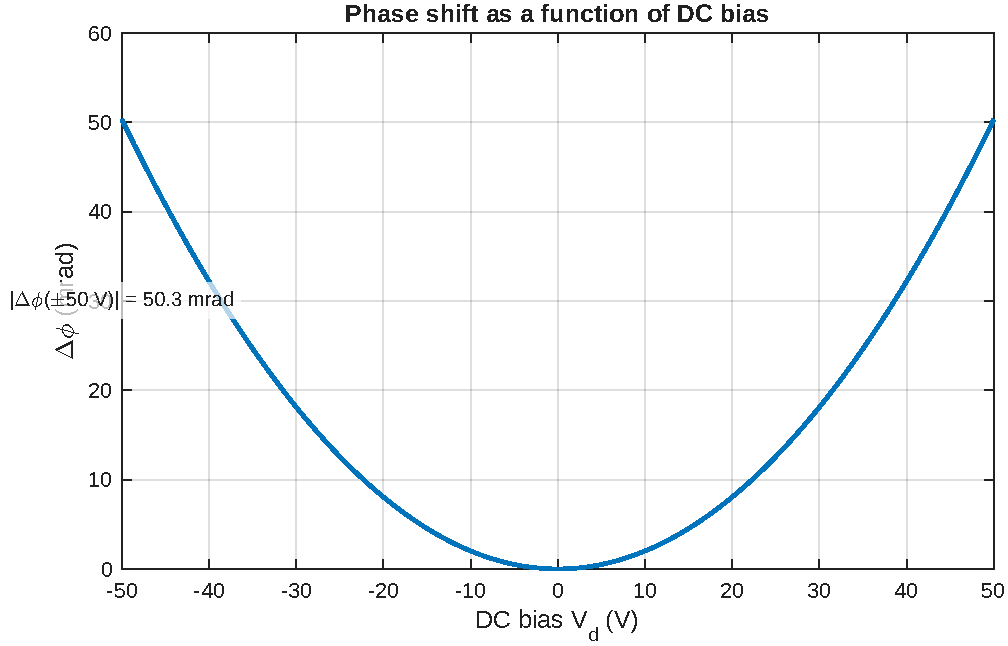
\includegraphics[width=0.78\textwidth]{figures/q6_phase_vs_V.pdf}
\caption{Static phase shift $\Delta\phi$ as a function of the DC bias
$\Vd\in[-50,\,+50]\,\mathrm{V}$. The shift is symmetric and quadratic in
$\Vd$, in line with Eq.~\ref{eq:Fcomb}.}
\label{fig:q6}
\end{figure}

\subsection*{Q7: Pull-in instability of the comb drive}

\paragraph{Case A, perpendicular field only.}
The overlap force in Eq.~\ref{eq:Fcomb} does not depend on $\xm$, so
$dF_{e}/d\xm = 0 < k$ for any $\Vd$. The single equilibrium
$\xm = \tfrac{1}{2}\Vd^{2}(dC/d\xm)/k$ is always stable. \emph{No pull-in.}
This is why comb drives are preferred over parallel-plate actuators when long
strokes are needed.

\paragraph{Case B, including finger-tip parallel-plate capacitance.}
When the mass moves into the comb, the gap between each finger tip and the
opposing anchor shrinks from $g_{t,0}=L_{c}-d_{0}=\SI{1}{\micro\meter}$ to
$g_{t}=g_{t,0}-\xm$. The additional capacitance and force per finger pair are
\begin{equation}
  C_{\mathrm{tip}}(\xm) = N\,\varepsilon_{0}\,\frac{W_{c}\,t}{g_{t,0}-\xm},
  \quad
  F_{\mathrm{tip}}(\xm) = \tfrac{1}{2}\,\Vd^{2}\,
                          \frac{N\,\varepsilon_{0}\,W_{c}\,t}{(g_{t,0}-\xm)^{2}}.
\end{equation}
Total force balance:
\begin{equation}
  k\xm = \tfrac{1}{2}\Vd^{2}\Biggl[\,
         \frac{N\varepsilon_{0}t}{h}
         + \frac{N\varepsilon_{0}W_{c}t}{(g_{t,0}-\xm)^{2}}\,\Biggr].
\end{equation}
Pull-in occurs when the small-signal stability condition $dF/d\xm = k$ is
reached:
\begin{equation}
  \Vd^{2}\,\frac{N\,\varepsilon_{0}\,W_{c}\,t}{(g_{t,0}-\xm)^{3}} = k.
\end{equation}
Eliminating $\Vd^{2}$ between the two equations gives an implicit relation
for the pull-in gap $u\equiv g_{t,0}-x_{\mathrm{pi}}$:
\begin{equation}
  g_{t,0} \;=\; \frac{3u}{2} + \frac{u^{3}}{2 h W_{c}}.
\end{equation}
Numerically, $u\approx\SI{0.60}{\micro\meter}$ (so
$x_{\mathrm{pi}}\approx\SI{0.40}{\micro\meter}$), giving the pull-in voltage
\begin{equation}
  V_{\mathrm{PI}} \;=\; \sqrt{\frac{k\,u^{3}}{N\,\varepsilon_{0}\,W_{c}\,t}}
                  \;\approx\; \SI{347}{\volt}.
\end{equation}
The mass-to-waveguide contact would only happen at
$\Vd \approx \sqrt{2 k g_{0}/(dC/d\xm)} \approx \SI{477}{\volt}$, so finger-tip
pull-in is what limits operation. As long as the bias stays well below
$\sim\!\SI{350}{\volt}$, Case A is a good model and the device behaves linearly.

\section{Small-signal modulation response}

\subsection*{Q8: Transfer function from $\VAC$ to $\Delta\phi$}

\paragraph{Linearised force.} With $\Vd(t)=\VDC + \VAC\sin(2\pi f_{m}t)$ and
$\VAC\ll \VDC$, the comb-drive force expands to first order as
\begin{align}
  \Fe &= \tfrac{1}{2}\,(\VDC+\VAC)^{2}\,\frac{dC}{d\xm}
       = \underbrace{\tfrac{1}{2}\VDC^{2}\frac{dC}{d\xm}}_{F_{\mathrm{DC}}}
         \;+\;
         \underbrace{\VDC\,\VAC\,\frac{dC}{d\xm}}_{f_{\mathrm{AC}}(t)}
         \;+\;\mathcal{O}(\VAC^{2}).
\end{align}
The AC component drives the small-signal motion with electromechanical
coupling
\begin{equation}
  \eta \;=\; \VDC\,\frac{dC}{d\xm} \;=\; \VDC\,\frac{N\,\varepsilon_{0}\,t}{h}.
  \label{eq:eta}
\end{equation}
The frequency response of the mass displacement is then
\begin{equation}
  \frac{X(s)}{V_{\!AC}(s)} \;=\; \frac{\eta}{m s^{2} + b s + k},
  \label{eq:Hxv}
\end{equation}
a standard second-order low-pass with poles at the resonance frequency.

\paragraph{Phase-shift sensitivity.} Linearising Eq.~\ref{eq:phase} around
the DC operating gap $g_{\mathrm{op}}=g_{0}+\xm(\VDC)$ via a first-order
Taylor expansion,
\begin{equation}
  \Delta\phi(g_{\mathrm{op}}+\delta g) \;\approx\;
  \Delta\phi(g_{\mathrm{op}})
    + \underbrace{\Bigl.\frac{d\Delta\phi}{dg}\Bigr|_{g_{\mathrm{op}}}}_{\equiv\,S_{\phi}}\,\delta g.
\end{equation}
Using $g=g_{0}+\xm$ so that $\delta g = \delta\xm$, and Eq.~\ref{eq:phase},
\begin{equation}
  \boxed{\;
  S_{\phi} \;=\; \frac{2\pi L}{\lambda}\,
                 (\eta_{\mathrm{eff},0}-\eta_{\mathrm{eff},\infty})\,
                 b\,e^{-b\,g_{\mathrm{op}}}.\;}
\end{equation}

\paragraph{Combined transfer function.} Multiplying Eq.~\ref{eq:Hxv} by
$S_{\phi}$ gives
\begin{equation}
  \boxed{\;
  H(s) \;=\; \frac{\Delta\phi(s)}{V_{\!AC}(s)}
        \;=\; \frac{S_{\phi}\,\eta}{m s^{2} + b s + k}.
  \;}
  \label{eq:Hphi}
\end{equation}

\paragraph{Performance metrics ($\VDC=\SI{10}{\volt}$).}
\begin{align}
  |H|_{f\to 0}     &= \frac{S_{\phi}\,\eta}{k}
                     \;\approx\; \SI{0.40}{\milli\radian\per\volt}, \\[2pt]
  |H|_{f=f_{0}}    &= \frac{S_{\phi}\,\eta\,Q}{k}
                     \;\approx\; \textcolor{blue}{\SI{33}{\milli\radian\per\volt}}
                     \;=\; Q\cdot|H|_{f\to 0}, \\[2pt]
  \text{roll-off} &= -\SI{40}{\decibel\per\text{decade}}\quad
                     \text{(two-pole low-pass above } f_{0}\text{)}.
\end{align}
Fig.~\ref{fig:bode} shows the Bode plot. The magnitude is flat below $f_{0}$,
peaks by $20\log_{10}Q\approx \textcolor{blue}{\SI{38}{\decibel}}$ at the lightly damped
resonance, then rolls off at $-40$\,dB/dec.

\begin{figure}[H]
\centering
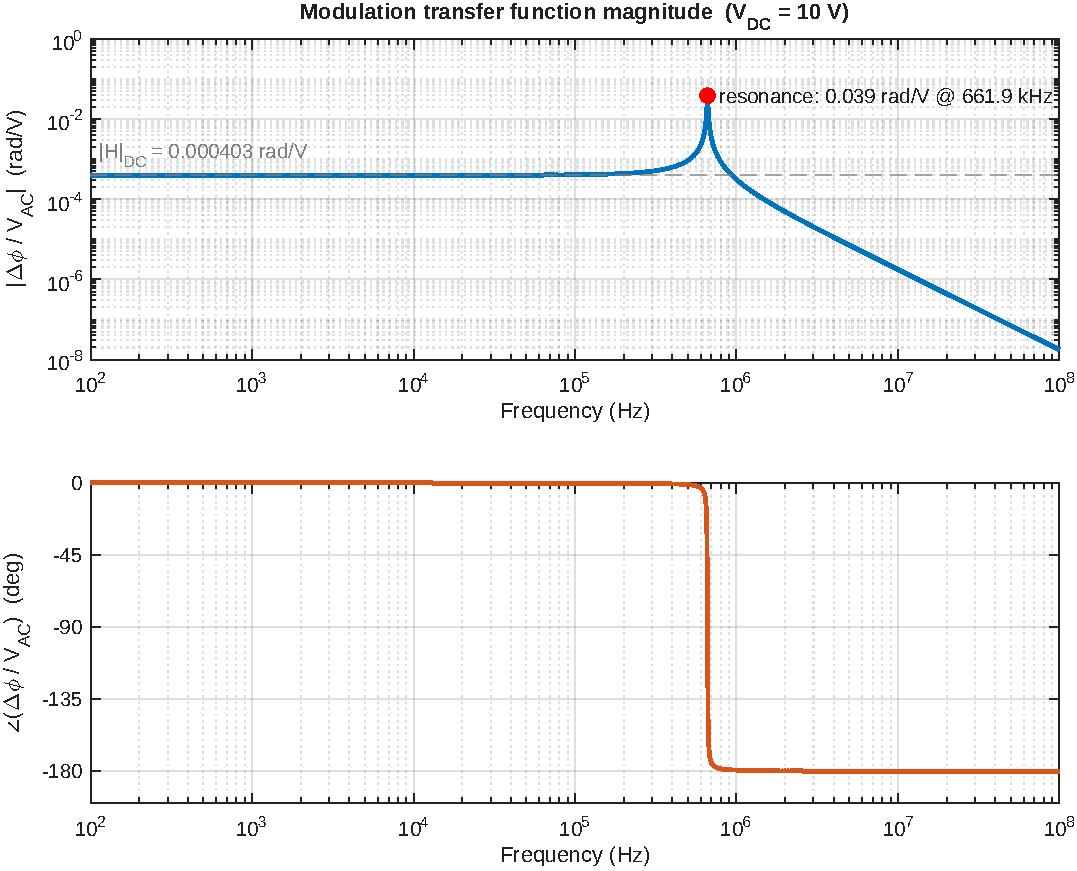
\includegraphics[width=0.85\textwidth]{figures/q8_bode.pdf}
\caption{Bode diagram of the small-signal transfer function
$\Delta\phi(s)/V_{\!AC}(s)$ at $\VDC=\SI{10}{\volt}$. The peak at
$f_{0}\approx\textcolor{blue}{\SI{537}{\kilo\hertz}}$ exceeds the low-frequency value by a
factor of $Q\approx \textcolor{blue}{81}$.}
\label{fig:bode}
\end{figure}

\paragraph{Low-frequency sensitivity vs DC bias.}
From Eqs.~\ref{eq:eta} and \ref{eq:Hphi},
$|H|_{f\to 0} = S_{\phi}\,\VDC\,(N\varepsilon_{0}t/h)/k \propto \VDC$ to first
order. Sensitivity scales linearly with $\VDC$ because $\eta$ does.
Fig.~\ref{fig:sensVDC} shows the response over $\VDC\in[0,\,5]\,\mathrm{kV}$,
with the linear small-signal prediction and the result that includes the
operating-point shift in $S_{\phi}$. Two practical limits are also marked:
finger-tip pull-in at $V_{\mathrm{PI}}\!\approx\!\SI{347}{\volt}$ and
mass-waveguide contact at $\!\approx\!\SI{477}{\volt}$. Above
$\sim\!\SI{350}{\volt}$ the device snaps down, so most of the plotted range
is unreachable in practice, it is shown only to illustrate the trend.

\begin{figure}[H]
\centering
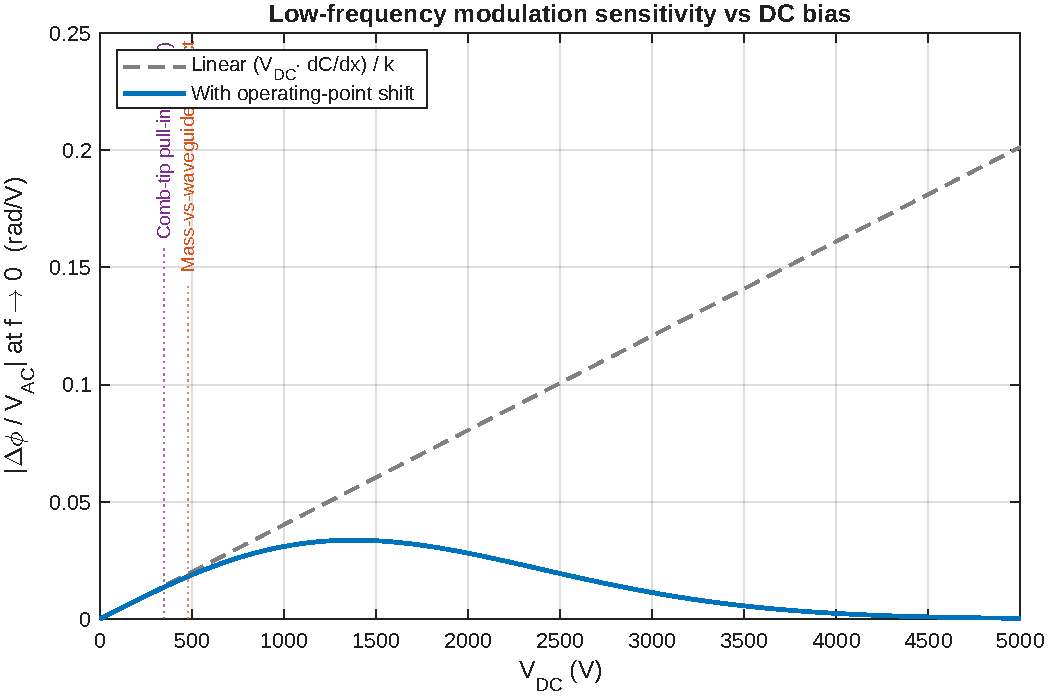
\includegraphics[width=0.78\textwidth]{figures/q8_sens_vs_VDC.pdf}
\caption{Low-frequency modulation sensitivity as a function of $\VDC$.
The dashed grey line is the strict linear $\VDC$ dependence; the solid line
includes the (small) effect of the operating-point shift on $S_{\phi}$.
Practical operation is bounded by comb-tip pull-in at $\sim\!\SI{347}{\volt}$.}
\label{fig:sensVDC}
\end{figure}

\section{Geometric scaling}

\subsection*{Q9 -- All dimensions multiplied by 1000}

Let every linear dimension grow by $\alpha=10^{3}$. Each derived quantity
picks up the corresponding power of $\alpha$ from its formula. Results are
collected in Table~\ref{tab:scaling}; the reasoning follows.

\begin{table}[H]
\centering
\small
\caption{Scaling of device characteristics for $\alpha=10^{3}$.}
\label{tab:scaling}
\begin{tabular}{l c c}
\toprule
\textbf{Quantity} & \textbf{Power of $\alpha$} & \textbf{Scale factor} \\
\midrule
Stiffness $k$              & $\alpha^{1}$  & $10^{3}$ \\
Effective mass $m$         & $\alpha^{3}$  & $10^{9}$ \\
Resonance $\omega_{0}=\sqrt{k/m}$ & $\alpha^{-1}$ & $10^{-3}$ \\
Gravity displacement $x_{g}=mg/k$ & $\alpha^{2}$  & $10^{6}$ \\
Max AC accel.\ $A_{\max,\mathrm{res}} = g_{0}\omega_{0}^{2}/Q$ & $\alpha^{-1}$ & $10^{-3}$ \\
Comb coupling $\eta = \VDC \, N\varepsilon_{0}\,t/h$ & $\alpha^{0}$ & $1$ \\
\bottomrule
\end{tabular}
\end{table}

\paragraph{Stiffness ($\propto \alpha$).}
$k = 4\,E_{Si}\,t\,W_{b}^{3}/L_{b}^{3}$ contains four lengths in the
numerator ($t,W_{b}^{3}$) and three in the denominator ($L_{b}^{3}$), so
$k \propto \alpha^{4-3} = \alpha$.

\paragraph{Mass ($\propto \alpha^{3}$).} $m = \rho\cdot V_{\mathrm{moving}}$ and
volume scales as $\alpha^{3}$.

\paragraph{Resonance ($\propto \alpha^{-1}$).}
$\omega_{0} = \sqrt{k/m} \propto \sqrt{\alpha/\alpha^{3}} = \alpha^{-1}$.
The macroscale device would resonate at $\sim \SI{660}{\hertz}$ instead of
$\SI{660}{\kilo\hertz}$.

\paragraph{Gravity displacement ($\propto \alpha^{2}$).}
$x_{g} = m g / k \propto \alpha^{3}/\alpha = \alpha^{2}$.
The $\SI{0.57}{\pico\meter}$ deflection becomes $\sim\!\SI{0.6}{\milli\meter}$.
Gravity, irrelevant here, becomes a dominant load at the macroscale.

\paragraph{Max AC acceleration ($\propto \alpha^{-1}$).}
$A_{\max,\mathrm{res}} = g_{0}\omega_{0}^{2}/Q \propto \alpha\cdot\alpha^{-2}
= \alpha^{-1}$ (assuming $Q$ unchanged). Shock tolerance drops from
$\sim\!3600\,g$ to a few $g$.

\paragraph{Coupling constant ($\alpha^{0}$).}
$\eta = \VDC\,N\,\varepsilon_{0}\,t/h$. With $N$ fixed and $t,h$ scaling
together, $t/h$ is invariant and $\eta$ stays the same at a given $\VDC$.

\bigskip
\noindent
The pattern is the usual one for MEMS: shrinking the device makes it stiffer
relative to its mass (faster), shock-tolerant, and immune to gravity. Going
in the opposite direction undoes all three.


\end{document}
